\documentclass[a4paper,conference]{IEEEtran}
\IEEEoverridecommandlockouts

\usepackage{cite}
\usepackage{amsmath,amssymb,amsfonts}
\usepackage{newtxtext,newtxmath}
\IfFileExists{local-fonts/times.ttf}{
  \newfontfamily\NTCIReferenceFont[Path=local-fonts/,Extension=.ttf,
    UprightFont=times,BoldFont=timesbd,ItalicFont=timesi,BoldItalicFont=timesbi]{times}
}{
  \newfontfamily\NTCIReferenceFont{Times New Roman}
}
\usepackage{graphicx}
\usepackage{textcomp}
\usepackage{xcolor}
\usepackage{geometry}
\usepackage{booktabs}
\usepackage{array}
\usepackage{url}
\usepackage{float}
\usepackage{multirow}
\usepackage{multicol}

\geometry{a4paper,left=2cm,right=2cm,top=2.5cm,bottom=4cm}

\newcommand{\fieldaligned}{Field-Aligned}
\newcommand{\conceptaligned}{Concept-Aligned}
\newcommand{\conceptclustered}{Concept-Clustered}
\newcommand{\fieldname}[1]{{\normalfont #1}}
\renewcommand{\figurename}{Fig.}
\renewcommand{\tablename}{Table}
\makeatletter
\renewcommand{\fnum@figure}{\figurename\thefigure}
\makeatother
\newcommand{\figref}[1]{\mbox{Fig.\ref{#1}}}
\newcommand{\tabref}[1]{\mbox{Table~\ref{#1}}}

\newcommand{\paperauthors}{%
Penghao~Shi\textsuperscript{1,6},
Yu~Cui\textsuperscript{2,6},
Yuxuan~Guo\textsuperscript{1,6},
Kanxue~Li\textsuperscript{3,6},
Da~Zhu\textsuperscript{2,6},
Shuo~Dang\textsuperscript{5,6},
Zhiyi~Yang\textsuperscript{2,6},
Jiarui~Wu\textsuperscript{1,6},
Yongcheng~Jing\textsuperscript{3},
Yibing~Zhan\textsuperscript{3},
Hua~Jin\textsuperscript{4},
Baodi~Liu\textsuperscript{1,7*},
Dapeng~Tao\textsuperscript{2},
Weifeng~Liu\textsuperscript{1}%
}

\newcommand{\paperaffiliations}{%
\textsuperscript{1}China University of Petroleum (East China), Qingdao 266580, Shandong, China\\
\textsuperscript{2}Yunnan University, Kunming 650500, Yunnan, China\\
\textsuperscript{3}Wuhan University, Wuhan 430072, Hubei, China\\
\textsuperscript{4}The First People's Hospital of Yunnan Province, Kunming 650032, Yunnan, China\\
\textsuperscript{5}Henan Normal University, Xinxiang 453007, Henan, China\\
\textsuperscript{6}Yunnan United Vision Technology Company Limited, Chenggong District, Kunming 650500, Yunnan, China\\
\textsuperscript{7}Qingdao Key Laboratory of Intelligent Sensing Technology for Extreme Environment%
}

\newcommand{\paperemails}{%
penghao\_shi@s.upc.edu.cn;
cuiyu@mail.ynu.edu.cn;
yuxuanguo@s.upc.edu.cn;
likanxue@whu.edu.cn\\
zhuda@mail.ynu.edu.cn;
dangshuo@stu.htu.edu.cn;
y15848899811@gmail.com\\
s24050026@upc.edu.cn;
ycjing@zju.edu.cn;
00036460@whu.edu.cn;
jinhuakm@163.com;
liubaodi@upc.edu.cn\\
dptao@ynu.edu.cn;
liuwf@upc.edu.cn%
}

\newcommand{\papercorrespondence}{%
Corresponding author: Baodi Liu; Email: liubaodi@upc.edu.cn%
}


\begin{document}

\title{Semantic Alignment of Heterogeneous Perioperative Data Resources for Computational Intelligence}

\author{
\IEEEauthorblockN{\parbox[t]{\textwidth}{\centering\paperauthors}}
\IEEEauthorblockA{\parbox[t]{\textwidth}{\centering\paperaffiliations}}
\IEEEauthorblockA{\papercorrespondence}
}

\maketitle

\begin{abstract}
Public perioperative resources cannot be pooled directly because their schemas and clinical values differ. We built a three-resource benchmark that first derives common preoperative fields and then maps 13 text fields to the Systematized Nomenclature of Medicine---Clinical Terms (SNOMED CT). Preprocessing produced 72,807 surgeries, a 58,553-record information-complete cohort, and a patient-grouped American Society of Anesthesiologists (ASA) physical status classification task with 28,397 records. Mapping generated 47,270 records covering 22,218 concepts. Concept alignment raised pairwise Jaccard overlap from 0.00--0.40\% to 2.40--3.82\% and increased the three-resource intersection from 2 source terms to 64 standardized concepts. In joint experiments using a clinical Bidirectional Encoder Representations from Transformers model (\mbox{ClinicalBERT}), mean Macro-F1 increased across six classifiers by 0.8--5.1\% relative to field alignment. Exploratory clustering reduced the concept space to 7,279 groups and raised overlap to 9.16--13.66\%, but rarely improved joint prediction beyond concept alignment. Field harmonization enabled joint computation; concept alignment added shared semantic support.
\end{abstract}

\vspace{\baselineskip}

\begin{IEEEkeywords}
\textit{perioperative data; semantic alignment; SNOMED CT; clinical benchmark; computational intelligence}
\end{IEEEkeywords}

\section{Introduction}
VitalDB, the Medical Informatics Operating Room Vitals and Events Repository (MOVER), and the Informative Surgical Patient dataset for Innovative Research Environment (INSPIRE) support perioperative risk research but differ in population, workflow, schema, and documentation~\cite{vitaldb,mover,inspire}. Our metadata-only audit found 3.51--7.32\% pairwise exact column-name overlap and incompatible keys, diagnoses, and clinical values, precluding direct concatenation.

Frameworks support intensive-care integration~\cite{ricu,yaib} and longitudinal evaluation~\cite{ehrshot}. Common data models and ontologies support schema conversion~\cite{ohdsi,snomed,umls}, and perioperative work mapped VitalDB, MOVER, and INSPIRE to the Observational Medical Outcomes Partnership Common Data Model (\mbox{OMOP-CDM}) with language-model assistance~\cite{kim_omop_perioperative}. Terminology normalization uses pairwise or neural ranking~\cite{dnorm,bert_normalization,n2c2}, domain-adapted encoders~\cite{clinicalbert}, retrieval-augmented generation (RAG)~\cite{rag}, and large language model (LLM) resolution~\cite{llm_snomed}. Incremental benefits of concept normalization and granularity reduction under a common patient-grouped perioperative protocol remain unclear.

We compare \fieldaligned{}, auditable Systematized Nomenclature of Medicine---Clinical Terms (\mbox{SNOMED CT}) \conceptaligned{}, and exploratory \conceptclustered{} representations using overlap, retrieval support, and patient-grouped American Society of Anesthesiologists (ASA) physical status prediction. We include independently sampled mapping review and licensed-data reconstruction boundaries, distinguishing computational interoperability from clinical validity.

\section{Benchmark Construction}
\subsection{Resources, Cohorts, and Patient-Level Splits}
Analysis-start cohorts contained 6,118 VitalDB, 21,990 MOVER, and 44,699 INSPIRE surgeries, after upstream exclusion of identified VitalDB--INSPIRE duplicate cases. A common filter required sex, age, height, weight, diagnosis, procedure, and either an organ-system history or five laboratory measurements, retaining 58,553 records. Extraction used VitalDB \fieldname{cases}, multiple MOVER \fieldname{epic\_emr} tables, and INSPIRE \fieldname{operations} and \fieldname{diagnosis} (\figref{fig:field-alignment}). Long-form laboratory normalization and pivoting produced 27 variables; diagnosis, procedure, medication, and history formed 13 text fields.

\onecolumn
\raggedbottom
\setlength{\multicolsep}{8pt}
\begin{multicols}{2}
\noindent Source keys were assigned to \fieldname{patient\_id} and \fieldname{surgery\_id}; residual identifiers and the resource indicator were excluded from predictors. Upstream processing removed 1,275 VitalDB-overlapping INSPIRE cases using \fieldname{case\_id} 1--6388. Laboratory events were selected preoperatively, cleaned, normalized by test name and unit, aggregated, and pivoted.

Seed-42 patient-grouped stratification retained 4,028 VitalDB, 12,236 MOVER, and 12,133 INSPIRE records (\tabref{tab:cohort-flow-full}). VitalDB lost 93 unlabeled records; MOVER and INSPIRE also had task-size caps, with label and sampling losses inseparable in available logs. All frozen splits had zero patient overlap. VitalDB contains ASA I--IV and the others I--V. VitalDB and INSPIRE share one hospital, limiting independent-site interpretation.
\end{multicols}
\begin{figure}[H]
\centering
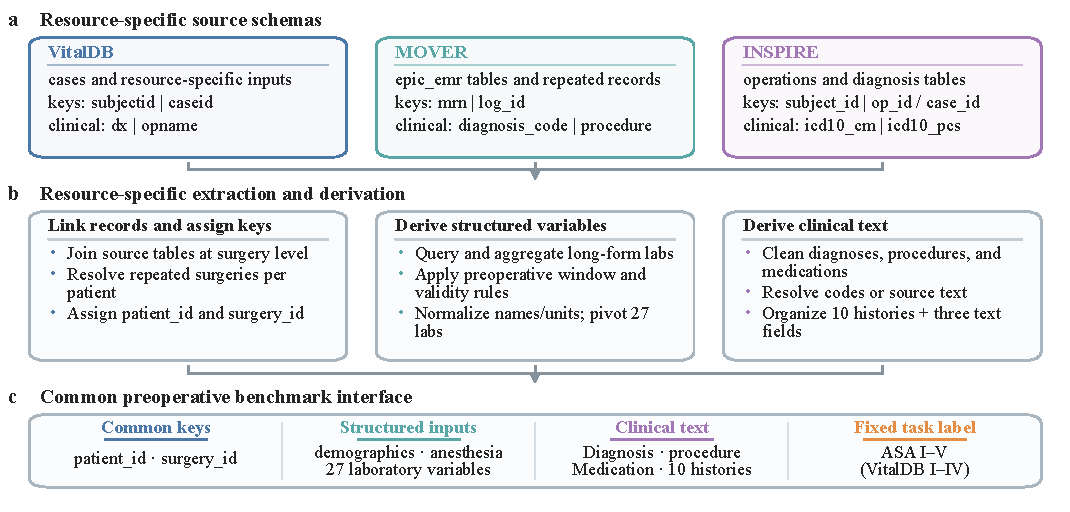
\includegraphics[width=\textwidth]{figures/fig01_field_alignment.pdf}
\caption{Field harmonization workflow. Resource-specific tables are linked by de-identified keys, laboratories are normalized into 27 variables, and clinical records are organized into 13 text fields. The common interface contains patient and surgery identifiers, structured inputs, text fields, and ASA labels; no identifier values or clinical records are shown.}
\label{fig:field-alignment}
\end{figure}
\begin{table}[H]
\caption{Cohort flow and final patient-grouped ASA splits.}
\label{tab:cohort-flow-full}
\centering\small
\begin{tabular}{lrrrrrr}
\toprule
Resource & Analysis start & Complete & ASA task & Train & Validation & Test \\
\midrule
VitalDB & 6,118 & 4,121 & 4,028 & 2,417 & 806 & 805 \\
MOVER & 21,990 & 17,129 & 12,236 & 7,308 & 2,460 & 2,468 \\
INSPIRE & 44,699 & 37,303 & 12,133 & 7,271 & 2,395 & 2,467 \\
Total & 72,807 & 58,553 & 28,397 & 16,996 & 5,661 & 5,740 \\
\bottomrule
\end{tabular}
\end{table}\begin{multicols}{2}
\subsection{SNOMED CT Alignment}
We standardized unique values from preoperative diagnosis, planned procedure, ten organ-system histories, and medication history against active descriptions in the 2026-02-01 SNOMED CT International Release. Exact strings scored 1.0. A frozen clinical Bidirectional Encoder Representations from Transformers model (\mbox{ClinicalBERT}; \fieldname{medicalai/ClinicalBERT}, 768 dimensions) and a Facebook AI Similarity Search (FAISS) index~\cite{faiss} retrieved 50 candidates. Vector similarity and bidirectional keyword coverage were weighted 0.8 and 0.2; listed negators zeroed keyword coverage, leaving $0.8\,\mathrm{sim}_{vec}$.

A hosted LLM received ambiguous terms with 15 candidates~\cite{rag}. This path used deepseek-v4-flash, temperature 0.1, high reasoning, and an 8,192-token limit; scores below 0.3 were rejected. Outputs retained identifier, name, mapping path, and automatic path-specific score (\figref{fig:overview}).

Resolving INSPIRE codes to English descriptions raised the fraction scoring $\geq0.85$ from 22.1\% to 93.4\% for the International Classification of Diseases, Tenth Revision, Clinical Modification (\mbox{ICD-10-CM}), and from 0.1\% to 69.1\% for the International Classification of Diseases, Tenth Revision, Procedure Coding System (\mbox{ICD-10-PCS}). \tabref{tab:icd-input-ablation} reports the full input ablation under the same mapper. All inputs received candidates; raw codes produced high-scoring lexical collisions. Representation-specific deduplication changed input counts, precluding paired comparison. Automatic scores are neither physician correctness estimates nor an official crosswalk.

The pipeline produced 47,270 mapping records. One physician reviewed a seed-42 sample of 30 records per resource--score stratum, except VitalDB's two low-score records (242 total). High meant exact match or score $\geq0.95$, middle $0.85\leq\mathrm{score}<0.95$, and low $<0.85$. Exact or broadly acceptable mappings totaled 170/242 (70.2\%, Wilson 95\% confidence interval (CI) 64.2--75.7\%). Weighting nine strata by population counts yielded 87.2\% acceptable (approximate 95\%~CI 80.6--93.7\%). Review did not change mappings; one reviewer and small low-score strata limit this estimate.
\end{multicols}
\begin{figure}[H]
\centering
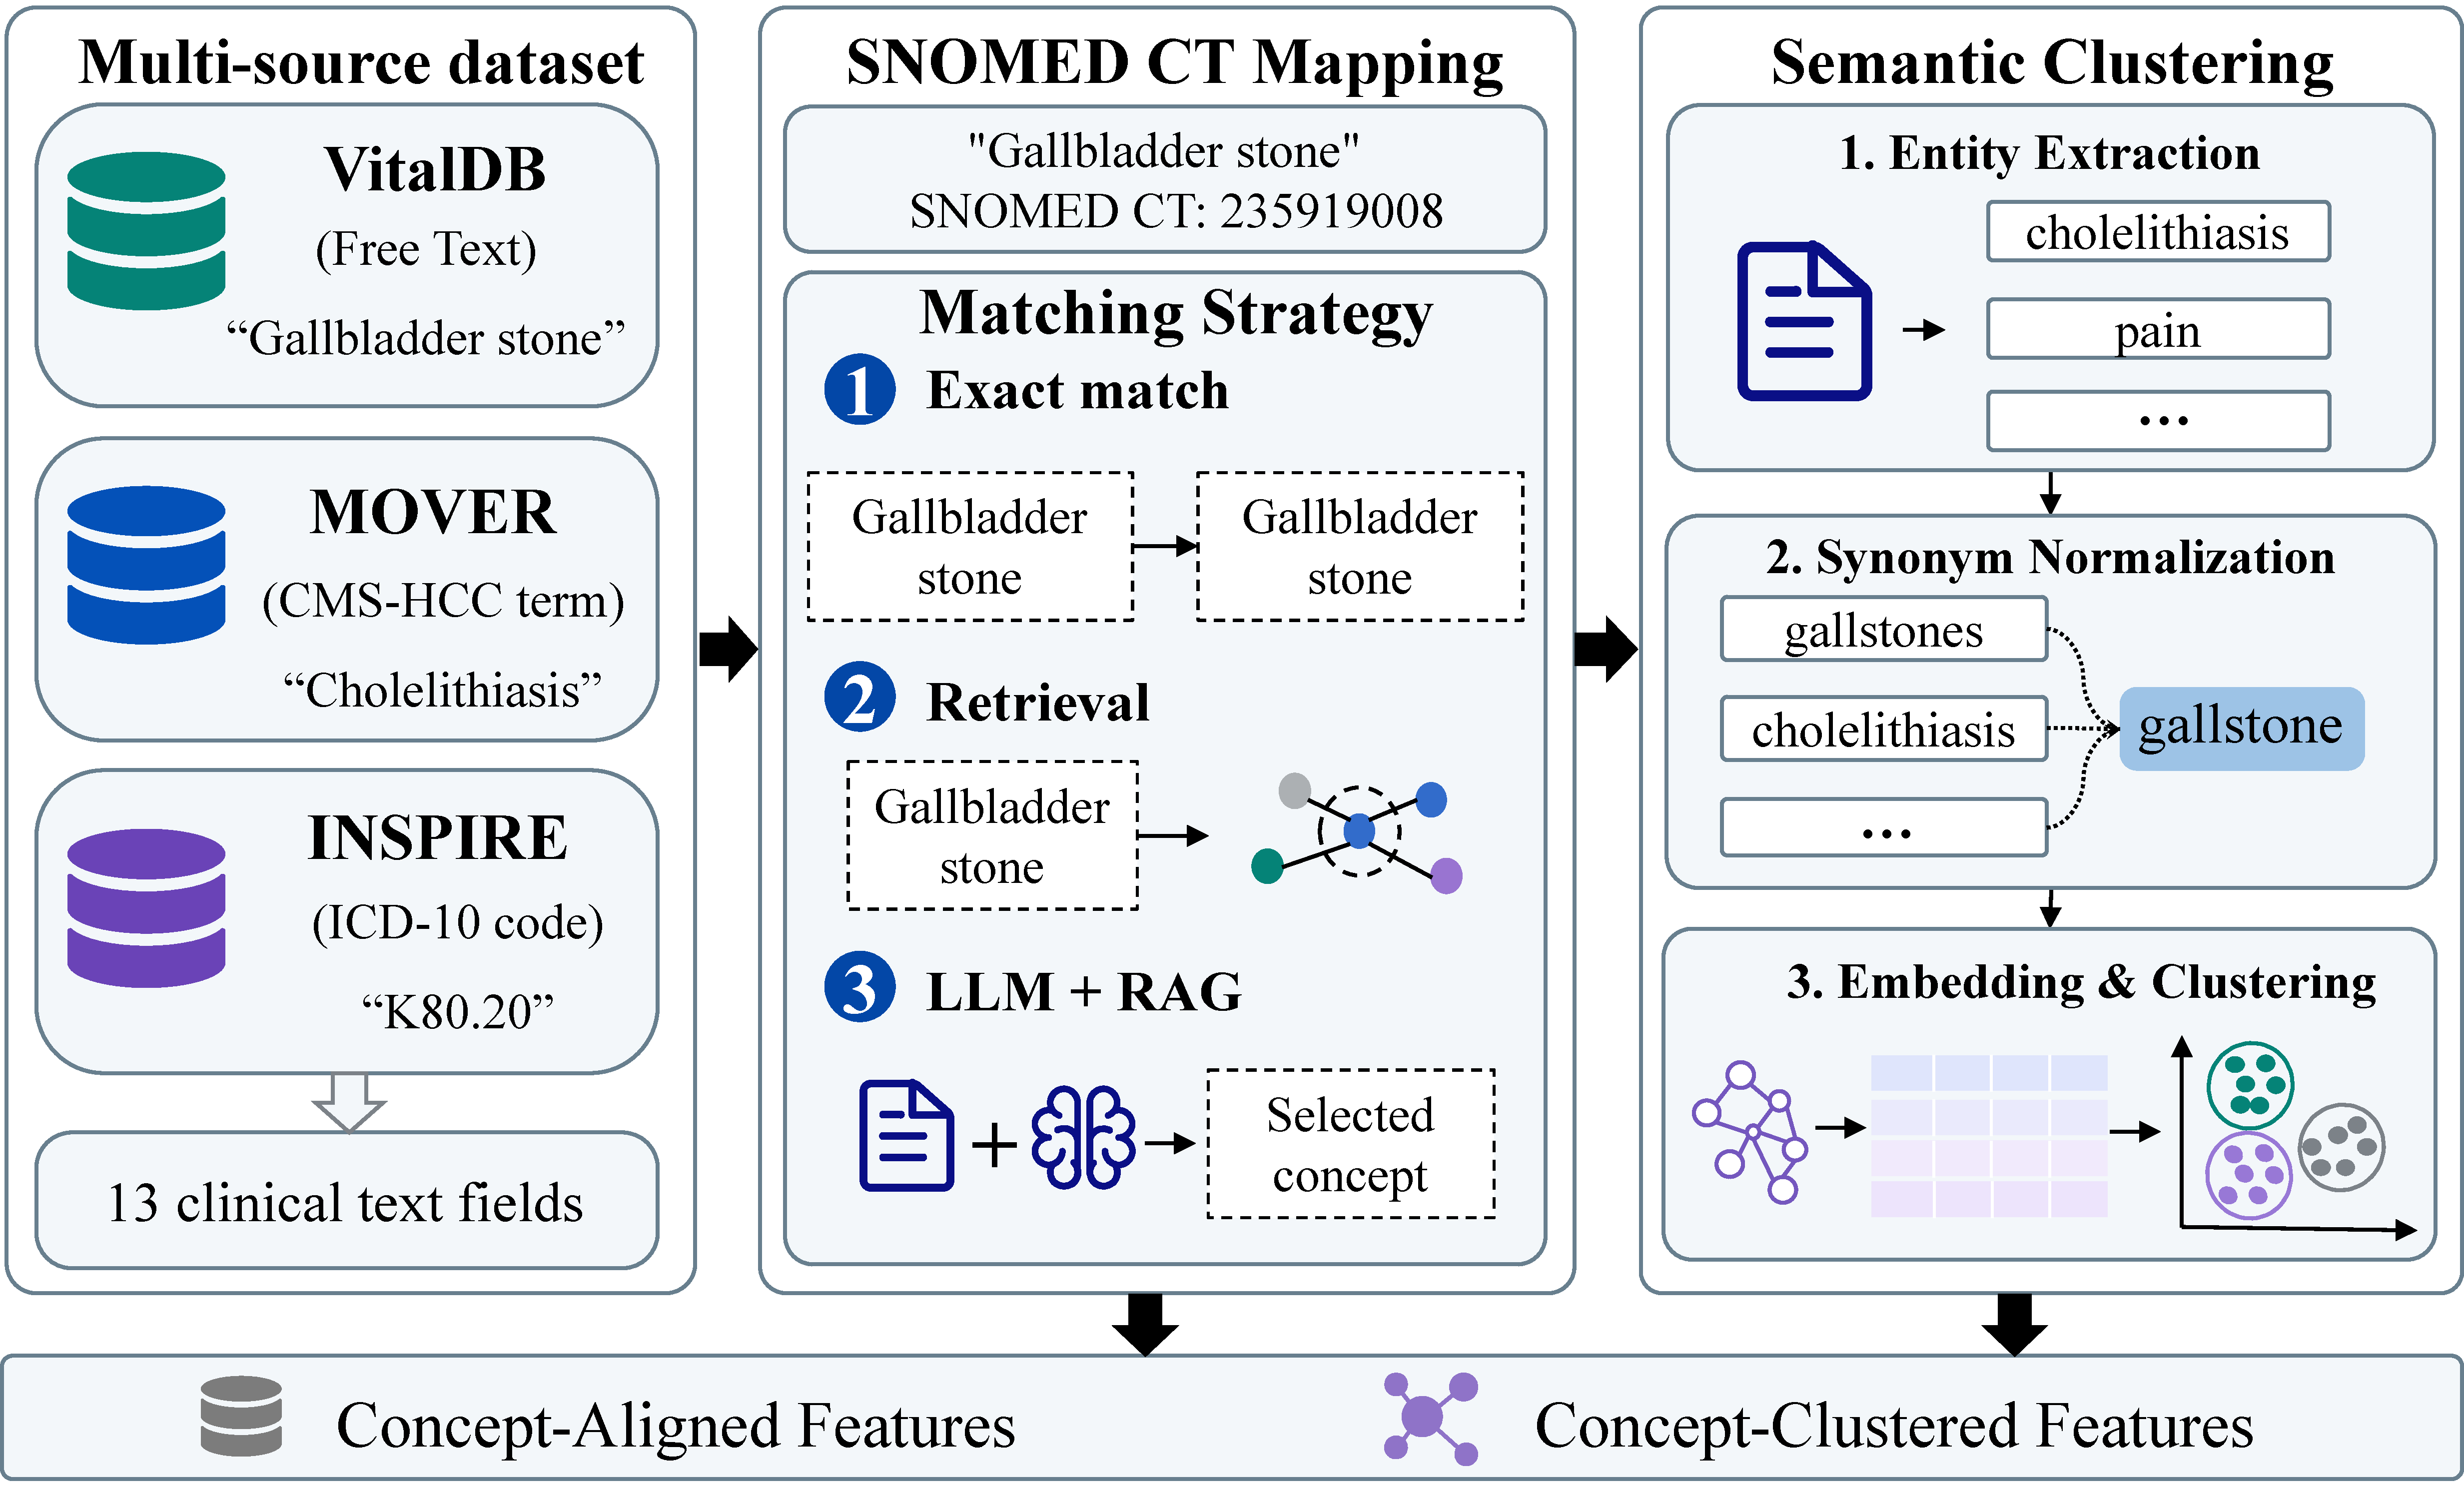
\includegraphics[width=0.85\textwidth]{figures/fig02_benchmark_overview.pdf}
\caption{Illustrative mapping and clustering workflow. Codes are resolved to English descriptions. LLM, large language model; RAG, retrieval-augmented generation; CMS-HCC, Centers for Medicare \& Medicaid Services Hierarchical Condition Category.}
\label{fig:overview}
\end{figure}
\begingroup
\renewenvironment{table*}[1][]{\begin{table}[H]}{\end{table}}
\begin{table*}[!t]
\caption{Code-versus-description ablation. Bold: improvement over raw codes. Score $\geq0.85$ is an automatic-score fraction, not physician-rated correctness.}
\label{tab:icd-input-ablation}
\centering\footnotesize
\setlength{\tabcolsep}{3.0pt}
\begin{tabular}{lllrrrrr}
\toprule
Subset & Code system & Mapper input & Unique $n$ & Exact (\%) & Retrieval (\%) & Mean score & Score $\geq0.85$ (\%) \\
\midrule
All unique inputs & ICD-10-CM & English description & 1,126 & \textbf{38.5} & 61.5 & \textbf{0.9494} & \textbf{93.4} \\
All unique inputs & ICD-10-CM & Raw code string & 765 & 0.9 & 99.1 & 0.8313 & 22.1 \\
All unique inputs & ICD-10-PCS & English description & 1,857 & \textbf{0.4} & 99.6 & \textbf{0.8640} & \textbf{69.1} \\
All unique inputs & ICD-10-PCS & Raw code string & 1,674 & 0.0 & 100.0 & 0.7613 & 0.1 \\
\midrule
Matched source-code set & ICD-10-CM & English description & 516 & \textbf{42.2} & 57.8 & \textbf{0.9561} & \textbf{96.1} \\
Matched source-code set & ICD-10-CM & Raw code string & 518 & 1.2 & 98.8 & 0.8309 & 20.5 \\
Matched source-code set & ICD-10-PCS & English description & 952 & \textbf{0.2} & 99.8 & \textbf{0.8648} & \textbf{69.8} \\
Matched source-code set & ICD-10-PCS & Raw code string & 1,054 & 0.0 & 100.0 & 0.7610 & 0.1 \\
\bottomrule
\end{tabular}
\end{table*}

\endgroup
\begin{multicols}{2}
\subsection{Granularity Reduction}
The 22,218 concepts were normalized using \fieldname{d4data/biomedical-ner-all}, SNOMED CT synonyms, and normalization rules, then \mbox{ClinicalBERT}-embedded and stratified by semantic type. Strata with $n>1{,}000$ used mini-batch k-means~\cite{minibatch_kmeans}: $k=\max(2,\min(\lfloor n/3\rfloor,5000))$, seed 42, three initializations, and 300 iterations. Smaller strata used Hierarchical Density-Based Spatial Clustering of Applications with Noise (\mbox{HDBSCAN})~\cite{hdbscan}, version 0.8.44, with minimum cluster size 5 and Euclidean distance. Pharmaceutical products used exact normalized strings. The most frequent member concepts named 7,279 clusters.

\end{multicols}
\clearpage
\begin{multicols}{2}
A size-weighted audit judged 20/30 sampled multi-member clusters consistent (66.7\%, Wilson 95\%~CI 48.8--80.8\%). Entropy-weighted identity retention was $\sum I(C;K)/\sum H(C)=91.8\%$ across ten positive-entropy resource--field combinations, where $C$ is concept identity, $K$ its cluster, $H$ entropy, and $I$ mutual information. This measures encoding, not clinical validity.

\subsection{Evaluation Inputs}
Joint ASA models used 768-dimensional \mbox{ClinicalBERT} text encodings and available structured variables. Categorical encoders and top-500-per-field one-hot vocabularies were fit on training data. \mbox{ClinicalBERT} used padding-masked mean pooling and averaged multi-valued fields. Numeric missingness was zero-filled without standardization. Mapping and clustering used full unlabeled vocabularies before splitting, making the representation comparison transductive.

\section{Evaluation Results}
\subsection{Shared Concept Space}
Within each surgery, text values were merged and deduplicated. Pairwise Jaccard overlap increased from \mbox{0.00--0.40\%} after field alignment to \mbox{2.40--3.82\%} after concept alignment and \mbox{9.16--13.66\%} after clustering (\figref{fig:concept}). The three-resource intersection contained 2 source terms, 64 concepts, and 167 clusters, whereas Jensen--Shannon divergence remained 0.530--0.761 after clustering.
\end{multicols}
\begin{figure}[H]
\centering
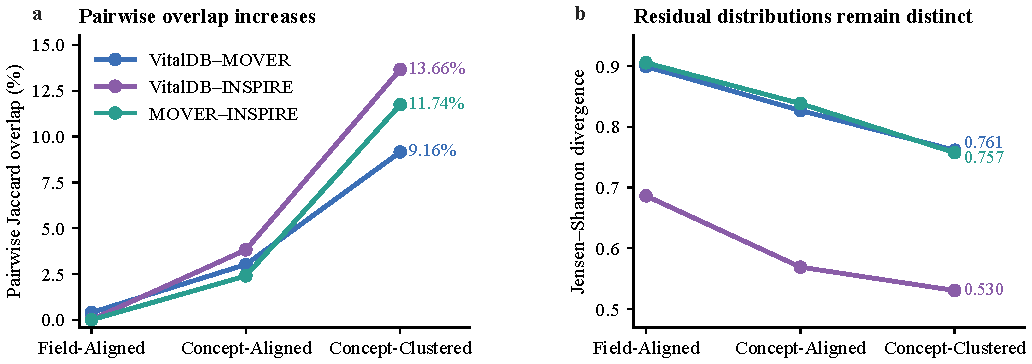
\includegraphics[width=0.97\textwidth]{figures/fig03_concept_space_tradeoff.pdf}
\caption{Pairwise concept overlap and residual distribution divergence. Jaccard overlap increases after concept alignment and clustering (a), whereas Jensen--Shannon divergence remains substantial (b).}
\label{fig:concept}
\end{figure}
\begin{multicols}{2}
\raggedcolumns
\subsection{Cross-Resource Retrieval}
Each resource's test split queried another resource's training split by cosine similarity over one-hot diagnosis, procedure, and history features. Zero-hit rate denotes queries with no shared feature. The four \fieldaligned{} directions involving INSPIRE had no shared feature, whereas both concept representations created support in all six directions (\figref{fig:retrieval}). Under \conceptclustered{}, zero-hit rates remained direction-dependent at 1.5--60.0\%.

\tabref{tab:knn-metrics-full} includes only non-zero queries, so representations evaluate different subsets. Accuracy and Macro-F1 (the unweighted mean of class-wise F1 scores) are auxiliary label-agreement measures. Fair accuracy divides accuracy by $1-r$, where $r$ is the fraction of queries with labels absent from the reference label space. Here $k$ is the number of neighbors; a dash denotes no eligible queries. Tied-vote handling was unidentified.

Coverage and label agreement thus characterize different aspects of cross-resource retrieval. Conditional scores exclude zero-hit queries, so they should be interpreted alongside the coverage rates.

\columnbreak
\subsection{ASA Model Readiness}
We evaluated logistic regression (LR)~\cite{cox_logistic}, random forests (RF)~\cite{breiman_rf}, extreme gradient boosting (\mbox{XGBoost})~\cite{xgboost}, multilayer perceptrons (MLP)~\cite{backprop}, one-dimensional convolutional neural networks (\mbox{1D-CNN})~\cite{lecun_cnn}, and TabTransformer~\cite{tabtransformer} over seeds 1--5 without task-specific tuning. \conceptaligned{} increased mean Macro-F1 by 0.0033--0.0209 (0.8--5.1\% relative) over \fieldaligned{} across all six classifiers (\figref{fig:model-readiness}). \conceptclustered{} exceeded \fieldaligned{} throughout but exceeded \conceptaligned{} only for LR. These small differences were not tested for statistical significance. \tabref{tab:joint-all} includes all six models and both encodings.

With one-hot inputs, concept alignment improved mean Macro-F1 only for RF and \mbox{1D-CNN} relative to field alignment. Clustering improved five of the six classifiers, with LR as the exception. Thus, the advantage of concept alignment across all six classifiers with \mbox{ClinicalBERT} did not extend uniformly to one-hot inputs. \mbox{ClinicalBERT} yielded higher mean Macro-F1 than one-hot inputs for every matched model--representation pair.
\end{multicols}
\begin{figure}[H]
\centering
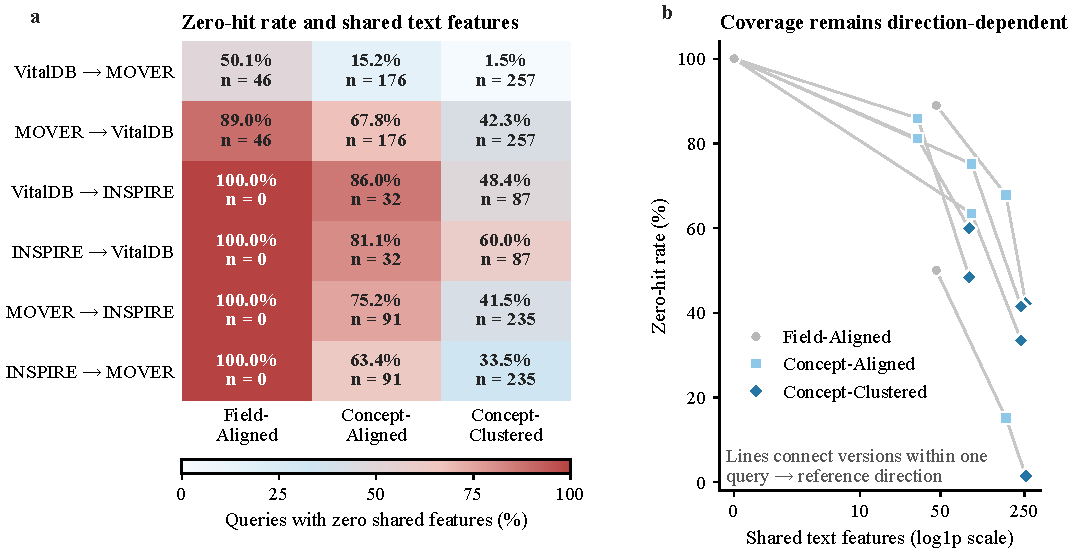
\includegraphics[width=0.96\textwidth]{figures/fig04_retrieval_coverage.pdf}
\caption{Six-direction retrieval coverage. Panel a reports zero-hit rates and shared-feature counts; panel b links the three representations within each query-to-reference direction. Concept alignment creates support in all directions, but coverage remains resource- and direction-dependent.}
\label{fig:retrieval}
\end{figure}
\begingroup
\renewenvironment{table*}[1][]{\begin{table}[H]}{\end{table}}
\begin{table*}[!t]
\caption{Retrieval-label agreement among non-zero queries. Acc., accuracy; fair acc., class-support-normalized accuracy; MF1, Macro-F1.}
\label{tab:knn-metrics-full}
\centering\footnotesize
\setlength{\tabcolsep}{1.8pt}
\begin{tabular}{llrrrrrrrrr}
\toprule
& & \multicolumn{3}{c}{$k=1$} & \multicolumn{3}{c}{$k=3$} & \multicolumn{3}{c}{$k=5$}\\
\cmidrule(lr){3-5}\cmidrule(lr){6-8}\cmidrule(lr){9-11}
Representation & Direction & Acc. & Fair acc. & MF1 & Acc. & Fair acc. & MF1 & Acc. & Fair acc. & MF1 \\
\midrule
Field-Aligned & INSPIRE $\rightarrow$ MOVER & -- & -- & -- & -- & -- & -- & -- & -- & -- \\
Field-Aligned & INSPIRE $\rightarrow$ VitalDB & -- & -- & -- & -- & -- & -- & -- & -- & -- \\
Field-Aligned & MOVER $\rightarrow$ INSPIRE & -- & -- & -- & -- & -- & -- & -- & -- & -- \\
Field-Aligned & MOVER $\rightarrow$ VitalDB & 0.2415 & 0.2435 & 0.1546 & 0.2605 & 0.2627 & 0.1630 & 0.2472 & 0.2492 & 0.1537 \\
Field-Aligned & VitalDB $\rightarrow$ INSPIRE & -- & -- & -- & -- & -- & -- & -- & -- & -- \\
Field-Aligned & VitalDB $\rightarrow$ MOVER & 0.3950 & 0.3950 & 0.1751 & 0.3801 & 0.3801 & 0.1774 & 0.4137 & 0.4137 & 0.1949 \\
Concept-Aligned & INSPIRE $\rightarrow$ MOVER & 0.2602 & 0.2602 & 0.1762 & 0.2084 & 0.2084 & 0.1456 & 0.2144 & 0.2144 & 0.1452 \\
Concept-Aligned & INSPIRE $\rightarrow$ VitalDB & 0.2619 & 0.2641 & 0.1603 & 0.2955 & 0.2980 & 0.1772 & 0.2910 & 0.2935 & 0.1746 \\
Concept-Aligned & MOVER $\rightarrow$ INSPIRE & 0.2314 & 0.2314 & 0.1572 & 0.2281 & 0.2281 & 0.1494 & 0.2180 & 0.2180 & 0.1430 \\
Concept-Aligned & MOVER $\rightarrow$ VitalDB & 0.2508 & 0.2529 & 0.1572 & 0.2857 & 0.2880 & 0.1697 & 0.2763 & 0.2786 & 0.1633 \\
Concept-Aligned & VitalDB $\rightarrow$ INSPIRE & 0.2571 & 0.2571 & 0.1641 & 0.2398 & 0.2398 & 0.1509 & 0.2261 & 0.2261 & 0.1504 \\
Concept-Aligned & VitalDB $\rightarrow$ MOVER & 0.3292 & 0.3292 & 0.1634 & 0.2360 & 0.2360 & 0.1434 & 0.2870 & 0.2870 & 0.1574 \\
Concept-Clustered & INSPIRE $\rightarrow$ MOVER & 0.2554 & 0.2554 & 0.1684 & 0.2469 & 0.2469 & 0.1598 & 0.2221 & 0.2221 & 0.1339 \\
Concept-Clustered & INSPIRE $\rightarrow$ VitalDB & 0.3247 & 0.3275 & 0.1849 & 0.3437 & 0.3467 & 0.1899 & 0.3685 & 0.3716 & 0.1834 \\
Concept-Clustered & MOVER $\rightarrow$ INSPIRE & 0.2776 & 0.2776 & 0.1688 & 0.2630 & 0.2630 & 0.1601 & 0.2557 & 0.2557 & 0.1481 \\
Concept-Clustered & MOVER $\rightarrow$ VitalDB & 0.2792 & 0.2815 & 0.1684 & 0.2901 & 0.2925 & 0.1642 & 0.3015 & 0.3039 & 0.1652 \\
Concept-Clustered & VitalDB $\rightarrow$ INSPIRE & 0.2559 & 0.2559 & 0.1545 & 0.2671 & 0.2671 & 0.1719 & 0.2932 & 0.2932 & 0.1721 \\
Concept-Clustered & VitalDB $\rightarrow$ MOVER & 0.2870 & 0.2870 & 0.1518 & 0.2571 & 0.2571 & 0.1385 & 0.2410 & 0.2410 & 0.1470 \\
\bottomrule
\end{tabular}
\end{table*}

\endgroup
\begingroup
\renewenvironment{table*}[1][]{\begin{table}[H]}{\end{table}}
\renewcommand{\arraystretch}{1.10}
\begin{table*}[!t]
\caption{Joint-training ASA Macro-F1 across all six models (mean $\pm$ standard deviation over five seeds). Bold: improvement over the matched Field-Aligned mean.}
\label{tab:joint-all}
\centering\footnotesize
\setlength{\tabcolsep}{2.4pt}
\begin{tabular}{llrrrrrr}
\toprule
Encoding & Representation & LR & RF & XGBoost & MLP & 1D-CNN & TabTransformer \\
\midrule
One-hot & Field-Aligned & $0.2470\pm0.0000$ & $0.2822\pm0.0024$ & $0.2809\pm0.0011$ & $0.2548\pm0.0003$ & $0.1944\pm0.0483$ & $0.2540\pm0.0013$ \\
One-hot & Concept-Aligned & $0.2429\pm0.0000$ & \textbf{0.2825}\,$\pm$\,\textbf{0.0026} & $0.2771\pm0.0021$ & $0.2545\pm0.0005$ & \textbf{0.1972}\,$\pm$\,\textbf{0.0475} & $0.2481\pm0.0070$ \\
One-hot & Concept-Clustered & $0.2461\pm0.0000$ & \textbf{0.2881}\,$\pm$\,\textbf{0.0029} & \textbf{0.2828}\,$\pm$\,\textbf{0.0043} & \textbf{0.2549}\,$\pm$\,\textbf{0.0001} & \textbf{0.2025}\,$\pm$\,\textbf{0.0412} & \textbf{0.2550}\,$\pm$\,\textbf{0.0001} \\
ClinicalBERT & Field-Aligned & $0.4002\pm0.0000$ & $0.4128\pm0.0057$ & $0.4804\pm0.0083$ & $0.2791\pm0.0128$ & $0.2250\pm0.0002$ & $0.3994\pm0.0127$ \\
ClinicalBERT & Concept-Aligned & \textbf{0.4035}\,$\pm$\,\textbf{0.0000} & \textbf{0.4337}\,$\pm$\,\textbf{0.0066} & \textbf{0.4914}\,$\pm$\,\textbf{0.0066} & \textbf{0.2924}\,$\pm$\,\textbf{0.0183} & \textbf{0.2316}\,$\pm$\,\textbf{0.0040} & \textbf{0.4083}\,$\pm$\,\textbf{0.0481} \\
ClinicalBERT & Concept-Clustered & \textbf{0.4101}\,$\pm$\,\textbf{0.0000} & \textbf{0.4262}\,$\pm$\,\textbf{0.0094} & \textbf{0.4821}\,$\pm$\,\textbf{0.0036} & \textbf{0.2816}\,$\pm$\,\textbf{0.0093} & \textbf{0.2305}\,$\pm$\,\textbf{0.0033} & \textbf{0.4022}\,$\pm$\,\textbf{0.0488} \\
\bottomrule
\end{tabular}
\end{table*}

\endgroup
\begin{figure}[H]
\centering
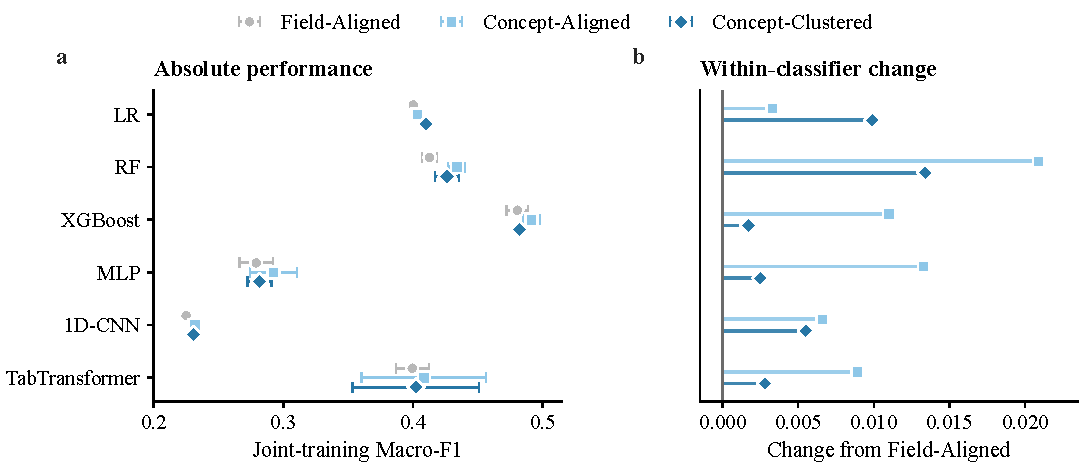
\includegraphics[width=0.88\textwidth]{figures/fig05_asa_model_readiness.pdf}
\caption{\mbox{ClinicalBERT} ASA results: five-seed mean Macro-F1 $\pm$ standard deviation (SD) (a), and change from \fieldaligned{} (b). LR, logistic regression; RF, random forest; MLP, multilayer perceptron; \mbox{1D-CNN}, one-dimensional convolutional neural network.}
\label{fig:model-readiness}
\end{figure}

\begin{multicols}{2}
\section{Discussion}
Field alignment enabled a common interface; concept alignment increased shared semantic support and produced small Macro-F1 gains in joint ClinicalBERT training; clustering increased overlap without uniform predictive gains.

These results establish computational interoperability, not clinical similarity. Resource distributions and directional zero-hit rates remained distinct. Although upstream preprocessing excluded identified duplicate cases, VitalDB and INSPIRE originate from the same hospital and do not provide independent-site validation. Raw diagnosis and procedure codes also produced lexical rather than semantic matches. Accordingly, \conceptaligned{} preserves auditable SNOMED CT identities, whereas \conceptclustered{} trades identity for coverage; the 91.8\% entropy-weighted concept-identity retention and 66.7\% cluster audit are not independent clinical validation.

Limitations include one mapping reviewer, 30 reviewed clusters, resource-specific preprocessing, and incomplete rerun reproducibility of the hosted language-model stage. Restricted frozen mappings permit downstream checks, but external reconstruction from released code and licensed sources may not reproduce identical mappings or results. Future work should add multiple reviewers, text-isolating ablations, and independent institutions.

\section{Reproducibility, Ethics, and Availability}
We analyzed released, de-identified data. Source approvals were VitalDB (H-1408-101-605), MOVER (2021-6488), and INSPIRE (H-2210-078-1368; BD-R-2022-11-02)~\cite{vitaldb,mover,inspire}. INSPIRE access required Collaborative Institutional Training Initiative (CITI) training and PhysioNet approval; no additional ethics approval was required.

Authorized users must acquire source data and SNOMED CT locally. Planned public artifacts comprise reconstruction/analysis code, task definitions, split logic, sanitized prompts/configurations, environment locks, aggregate evidence, and snapshot hashes. Source records, patient-level features/predictions/split maps, term-level mappings, clusters, and licensed ontology assets are excluded. Frozen mappings permit restricted downstream replay; raw hosted-model responses were not retained, and rerunning that stage or public reconstruction need not reproduce identical outputs.

\section{Conclusion}
Concept alignment increased shared support and slightly improved joint ClinicalBERT Macro-F1; clustering improved coverage without uniform predictive gains. Resource differences, limited audits, and absent independent external validation constrain these findings.

\section*{Acknowledgment}
This work is supported by the Yunnan Provincial Key Science and Technology Project (Grant No. 202502AS080002); the Yunling Scholar Talent Program of Yunnan Province (Grant No. K264202230207); Shandong Natural Science Foundation (ZR2024MF102); Fundamental Research Funds for the Central Universities, China University of Petroleum (East China) (26CX02005A); Qingdao Key Laboratory of Intelligent Sensing Technology for Extreme Environment (2025YB001); Key Projects of the Qingdao Natural Science Foundation (25-3-1-3-zyyd-jch); Major Basic Research Projects in Shandong Province (ZR2023ZD32); Open Project of Yunnan Key Laboratory of Media Convergence (ynmckey220252201); and Zhejiang Province Leading Earth Goose Program (2025C01129).

\end{multicols}
\clearpage
\begin{multicols}{2}
\begingroup
\footnotesize
\NTCIReferenceFont
\begin{thebibliography}{25}
\interlinepenalty=10000

\bibitem{vitaldb}
H.-C. Lee, Y. Park, S.-B. Yoon, \emph{et al.}, ``VitalDB, a high-fidelity multi-parameter vital signs database in surgical patients,'' \emph{Scientific Data}, 9: 279, 2022.

\bibitem{mover}
M. Samad, M. Angel, J. Rinehart, \emph{et al.}, ``Medical Informatics Operating Room Vitals and Events Repository (MOVER): a public-access operating room database,'' \emph{JAMIA Open}, 6(4): ooad084, 2023.

\bibitem{inspire}
L. Lim, H. Lee, C.-W. Jung, \emph{et al.}, ``INSPIRE, a publicly available research dataset for perioperative medicine,'' \emph{Scientific Data}, 11: 655, 2024.

\bibitem{ricu}
N. Bennett, D. Ple\v{c}ko, I.-F. Ukor, \emph{et al.}, ``ricu: R's interface to intensive care data,'' \emph{GigaScience}, 12: giad041, 2023.

\bibitem{yaib}
R. van de Water, H. Schmidt, P. Elbers, \emph{et al.}, ``Yet Another ICU Benchmark: a flexible multi-center framework for clinical ML,'' in \emph{Proceedings of the 12th International Conference on Learning Representations (ICLR)}. Vienna, Austria: OpenReview, 2024.

\bibitem{ehrshot}
M. Wornow, R. Thapa, E. Steinberg, \emph{et al.}, ``EHRSHOT: an EHR benchmark for few-shot evaluation of foundation models,'' in \emph{Advances in Neural Information Processing Systems}, 36: 67125--67137. New Orleans, LA, USA: Curran Associates, Inc., 2023.

\bibitem{ohdsi}
G. Hripcsak, J. D. Duke, N. H. Shah, \emph{et al.}, ``Observational Health Data Sciences and Informatics (OHDSI): opportunities for observational researchers,'' in \emph{MEDINFO 2015: eHealth-enabled Health, Proceedings of the 15th World Congress on Health and Biomedical Informatics}, 216: 574--578. S\~ao Paulo, Brazil: IOS Press, 2015, doi: 10.3233/978-1-61499-564-7-574.

\bibitem{snomed}
SNOMED International, ``What is SNOMED CT?,'' website. [Online]. Available: \url{https://www.snomed.org/what-is-snomed-ct}. Accessed: Aug. 22, 2026.

\bibitem{umls}
O. Bodenreider, ``The Unified Medical Language System (UMLS): integrating biomedical terminology,'' \emph{Nucleic Acids Research}, 32(suppl. 1): D267--D270, 2004.

\bibitem{kim_omop_perioperative}
H. Kim, H. Lee, D. Lee, \emph{et al.}, ``Harmonizing perioperative open datasets using the OMOP-CDM via LLM and LangChain,'' conference presentation at the 10th OHDSI Global Symposium, New Brunswick, NJ, USA, Oct. 22--24, 2024. [Online]. Available: \url{https://www.ohdsi.org/wp-content/uploads/2024/12/8b.-LLM-and-OHDSI-Part-2_Hyeonsik-Kim.pdf}. Accessed: Aug. 22, 2026.

\bibitem{dnorm}
R. Leaman, R. Islamaj Do\u{g}an, and Z. Lu, ``DNorm: disease name normalization with pairwise learning to rank,'' \emph{Bioinformatics}, 29(22): 2909--2917, 2013.

\bibitem{bert_normalization}
Z. Ji, Q. Wei, and H. Xu, ``BERT-based ranking for biomedical entity normalization,'' in \emph{AMIA Joint Summits on Translational Science Proceedings}, pp. 269--277. Bethesda, MD, USA: American Medical Informatics Association, 2020.

\bibitem{n2c2}
Y.-F. Luo, S. Henry, Y. Wang, \emph{et al.}, ``The 2019 n2c2/UMass Lowell shared task on clinical concept normalization,'' \emph{Journal of the American Medical Informatics Association}, 27(10): 1529--e1, 2020, doi: 10.1093/jamia/ocaa106.

\bibitem{clinicalbert}
E. Alsentzer, J. R. Murphy, W. Boag, \emph{et al.}, ``Publicly available clinical BERT embeddings,'' in \emph{Proceedings of the 2nd Clinical Natural Language Processing Workshop}, pp. 72--78. Minneapolis, MN, USA: Association for Computational Linguistics, 2019.

\bibitem{rag}
P. Lewis, E. Perez, A. Piktus, \emph{et al.}, ``Retrieval-augmented generation for knowledge-intensive NLP tasks,'' in \emph{Advances in Neural Information Processing Systems}, 33: 9459--9474. Red Hook, NY, USA: Curran Associates, Inc., 2020.

\bibitem{llm_snomed}
S. Huh, ``Comparative analysis of ChatGPT-4 for automated mapping of local medical terminologies to SNOMED CT,'' in \emph{Intelligent Health Systems---From Technology to Data and Knowledge: Proceedings of MIE 2025}, 327: 813--817. Glasgow, UK: IOS Press, 2025, doi: 10.3233/SHTI250472.

\bibitem{faiss}
J. Johnson, M. Douze, and H. J\'egou, ``Billion-scale similarity search with GPUs,'' \emph{IEEE Transactions on Big Data}, 7(3): 535--547, 2021.

\bibitem{minibatch_kmeans}
D. Sculley, ``Web-scale K-means clustering,'' in \emph{Proceedings of the 19th International Conference on World Wide Web}, pp. 1177--1178. Raleigh, NC, USA: Association for Computing Machinery, 2010.

\bibitem{hdbscan}
R. J. G. B. Campello, D. Moulavi, and J. Sander, ``Density-based clustering based on hierarchical density estimates,'' in \emph{Advances in Knowledge Discovery and Data Mining: PAKDD 2013, Part II}, \emph{Lecture Notes in Computer Science}, 7819: 160--172. Gold Coast, QLD, Australia: Springer Berlin Heidelberg, 2013.

\bibitem{cox_logistic}
D. R. Cox, ``The regression analysis of binary sequences,'' \emph{Journal of the Royal Statistical Society: Series B (Methodological)}, 20(2): 215--232, 1958.

\bibitem{breiman_rf}
L. Breiman, ``Random forests,'' \emph{Machine Learning}, 45(1): 5--32, 2001.

\bibitem{xgboost}
T. Chen and C. Guestrin, ``XGBoost: a scalable tree boosting system,'' in \emph{Proceedings of the 22nd ACM SIGKDD International Conference on Knowledge Discovery and Data Mining}, pp. 785--794. San Francisco, CA, USA: Association for Computing Machinery, 2016.

\bibitem{backprop}
D. E. Rumelhart, G. E. Hinton, and R. J. Williams, ``Learning representations by back-propagating errors,'' \emph{Nature}, 323: 533--536, 1986.

\bibitem{lecun_cnn}
Y. LeCun, L. Bottou, Y. Bengio, \emph{et al.}, ``Gradient-based learning applied to document recognition,'' \emph{Proceedings of the IEEE}, 86(11): 2278--2324, 1998.

\bibitem{tabtransformer}
X. Huang, A. Khetan, M. Cvitkovic, \emph{et al.}, ``TabTransformer: tabular data modeling using contextual embeddings,'' arXiv preprint arXiv:2012.06678, 2020.

\end{thebibliography}

\endgroup
\end{multicols}

\end{document}
